\documentclass[11pt]{article}
\usepackage[a4paper,margin=2.6cm]{geometry}
\usepackage[T1]{fontenc}
\usepackage[utf8]{inputenc}
\usepackage{lmodern}
\usepackage{microtype}
\usepackage{booktabs}
\usepackage{graphicx}
\usepackage{amsmath}
\usepackage[hidelinks]{hyperref}
\usepackage{natbib}
\bibliographystyle{unsrtnat}
\usepackage{caption}
\captionsetup{font=small,labelfont=bf}

\title{\textbf{EXTRAI-2: with a deterministic harness, reading is the whole game --- five small local language models as the sole model stage of a meta-analysis pipeline}}
\author{Gustavo Barcelos Barra\thanks{Independent researcher, Brazil. ORCID: \href{https://orcid.org/0000-0002-2136-3471}{0000-0002-2136-3471}. Correspondence: \texttt{gbbarra@gmail.com}.}}
\date{August 2026}

\begin{document}
\maketitle

\begin{abstract}
\noindent In the companion EXTRAI benchmark, small local language models proved reviewer-grade readers and, given a calculator, reviewer-grade statisticians --- but undisciplined assemblers: a chained pipeline's quality gate caused six times more pooled-estimate damage than the sabotage it caught, and no model reliably orchestrated its own tools. This second study takes that measured conclusion as a design principle: everything deterministic moves into pre-registered, frozen code, and the model under test keeps only what requires reading. One question was frozen before any run: can local models that fit on an integrated GPU reach a published meta-analytic value --- an HbA1c mean difference of $-0.24$ $[-0.32, -0.16]$ under low-carbohydrate diets --- when extraction is theirs and everything downstream is code? Five quantized open-weight models (8--14.8B parameters, consumer mini-PC, no discrete GPU, no cloud API calls) each read the seven perturbed primary trials from zero; a deterministic engine selected field routes, converted dispersions, computed every effect and pooled them; mechanically detected judgment triggers asked the extractor one narrow, logged question each. The answer is yes --- for exactly one model. \texttt{gemma4:12b}'s unperturbed diamond lands beside the published value ($-0.27$ $[-0.38, -0.17]$; $-0.24$ to the hundredth in its first round), while the other four land between $-0.44$ and $-0.54$ for \emph{named reading failures} --- a unit-and-level chimera, values computed instead of read, a wrong timepoint, and the benchmark's first outright inventions --- never for arithmetic: every pipeline pool equals an independent recomputation over the same sheets, two of five digit for digit. An A/B across rounds showed a judgment ``failure'' vanish when a leading trigger question was made neutral: instruments, not only models, create failure modes. With the harness closed, reading is the whole game --- and among iGPU-scale models today, exactly one plays it well enough. All protocols, amendments, seals, sheets, graders and adjudications are public and archived.
\end{abstract}

\section{Introduction}

The companion study \citep{barra2026companion} chained four small local language models into an autonomous meta-analysis pipeline and measured where it broke. The models read almost perfectly (one wrong cell in 624), computed perfectly through a trivial text-protocol calculator (8/8 point estimates and intervals), and still delivered a distorted diamond --- because the connective tissue failed: an auditing model ``repaired'' correct cells, a calculating model flipped the sign of a value it disliked, a pooling call was fed dispersions inconsistent with the same model's own per-study calls, and syntheses summed participant counts mentally and got both sums wrong. The pipeline's quality gate did six times more damage to the pooled estimate than the planted sabotage it was hired to catch.

There are two possible responses to that finding. One is to search for a model disciplined enough to orchestrate. The other is to stop asking models to orchestrate at all. This study measures the second response, taken to its limit: \textbf{every deterministic operation --- field routing, dispersion conversion, effect computation, pooling --- moves into pre-registered, frozen code, and the model under test keeps exactly one job, the one that irreducibly requires reading}. The design question this isolates was frozen in the protocol before any run:

\begin{quote}
\emph{Can local models that fit on an integrated GPU reach the expected meta-analytic value --- the published $-0.24$ $[-0.32, -0.16]$ --- when extraction is theirs and everything downstream is deterministic code?}
\end{quote}

The study contributes: (1) a \textbf{measured ladder} of harness designs, from spontaneous model discipline to code-owned orchestration, showing failure modes migrating upward until only reading remains; (2) a \textbf{deterministic pipeline architecture} with mechanically detected \emph{judgment triggers} --- narrow, logged questions the extractor itself answers when its sheet presents a genuine reading judgment; (3) a five-extractor measurement whose central result is that \textbf{in-world exactness and fidelity to the literature are independent axes} --- a pipeline can equal the mechanical truth of its own sheets digit for digit while its sheets describe a world that never existed; (4) an \textbf{instrument A/B} in which a judgment failure observed under a leading question disappears under a neutral one --- evidence that evaluation instruments manufacture failure modes; and (5) a \textbf{failure taxonomy} of small extractors, including the benchmark's first outright inventions, grounded cell by cell in source quotes.

\section{Inherited constitution}

The corpus, instruments and grading doctrine are the companion study's, unchanged \citep{barra2026companion}. The anchor is a recent meta-analysis of low-carbohydrate diets for glycemic control in type~2 diabetes \citep{khraise2026lowcarb} with its seven primary randomized trials. Before any model reads a trial, a sealed, deterministic operator displaces load-bearing numbers in its text (the \emph{perturbation reading proof}): a model that returns the displaced value read the text; one that returns the published value recited training data \citep{xu2024contamination}. Sheets are graded against a \emph{two-layer answer key} verified against the primary sources, with a literal quote recorded per decision; ambiguous cells go to an adjudication rite that obliges the judge to quote the source before deducting, and the adjudicator's own errors are published as errata. The extraction instrument (a structured Portuguese sheet per trial: means, dispersions, group sizes, and the \emph{declared type} of each dispersion) is frozen from the companion study; changes to anything are possible only as dated protocol amendments registered before the runs they govern. All computation runs on one consumer mini-PC (AMD Ryzen~7, 780M integrated GPU, 32~GB RAM) through Ollama, with exact quantized builds pinned by digest in the archived repository; no cloud API is called anywhere in the evaluated pipelines.

\section{The ladder: how orchestration failures migrated into code}

Four pre-registered arms, run between the companion study and this one, motivate the design (each is a one-line summary of a fully archived record):

\begin{itemize}
  \item \textbf{Spontaneous discipline} (the companion's cast and an all-\texttt{gemma4:12b} cast): the small models fail at workflow --- the all-12B pipeline \emph{inverted} the diamond to $+0.85$ by answering by head, and an iGPU cast died at the tool loop's mixed-round joint.
  \item \textbf{Flow nets} (a harness that policed the tool loop): the workflow failures disappeared --- tool used, pool reconciled, loop closed --- and the diamond was still wrong ($+0.37$), because the nets cannot reach \emph{content}: the model assembled correct calls from sign-corrupted arguments.
  \item \textbf{Audit committees}: pooling two auditors' verdicts by OR repaired 10/10 seeded errors, and the 27B calculator over those committee-repaired sheets reproduced the sheets' mechanical truth digit for digit --- proof that the \emph{sheets} support an exact diamond when orchestration is taken away from chance.
  \item \textbf{Code-owned orchestration}: with the harness owning everything deterministic and models consulted only at judgment points, all arms reproduced the mechanical truth digit for digit ($-0.52$ $[-0.82, -0.22]$) --- and on that corpus, zero judgment triggers fired: model necessity had concentrated entirely at extraction.
\end{itemize}

The ladder's lesson is monotone: every rung moves a class of failure out of the model and into code, and the failures that remain are reading failures. Study 4 --- this paper's measurement --- makes the remaining stage the experiment: \emph{fresh} extraction from zero, by five different models, under the identical deterministic downstream.

\section{Design}

\begin{figure}[t]
\centering
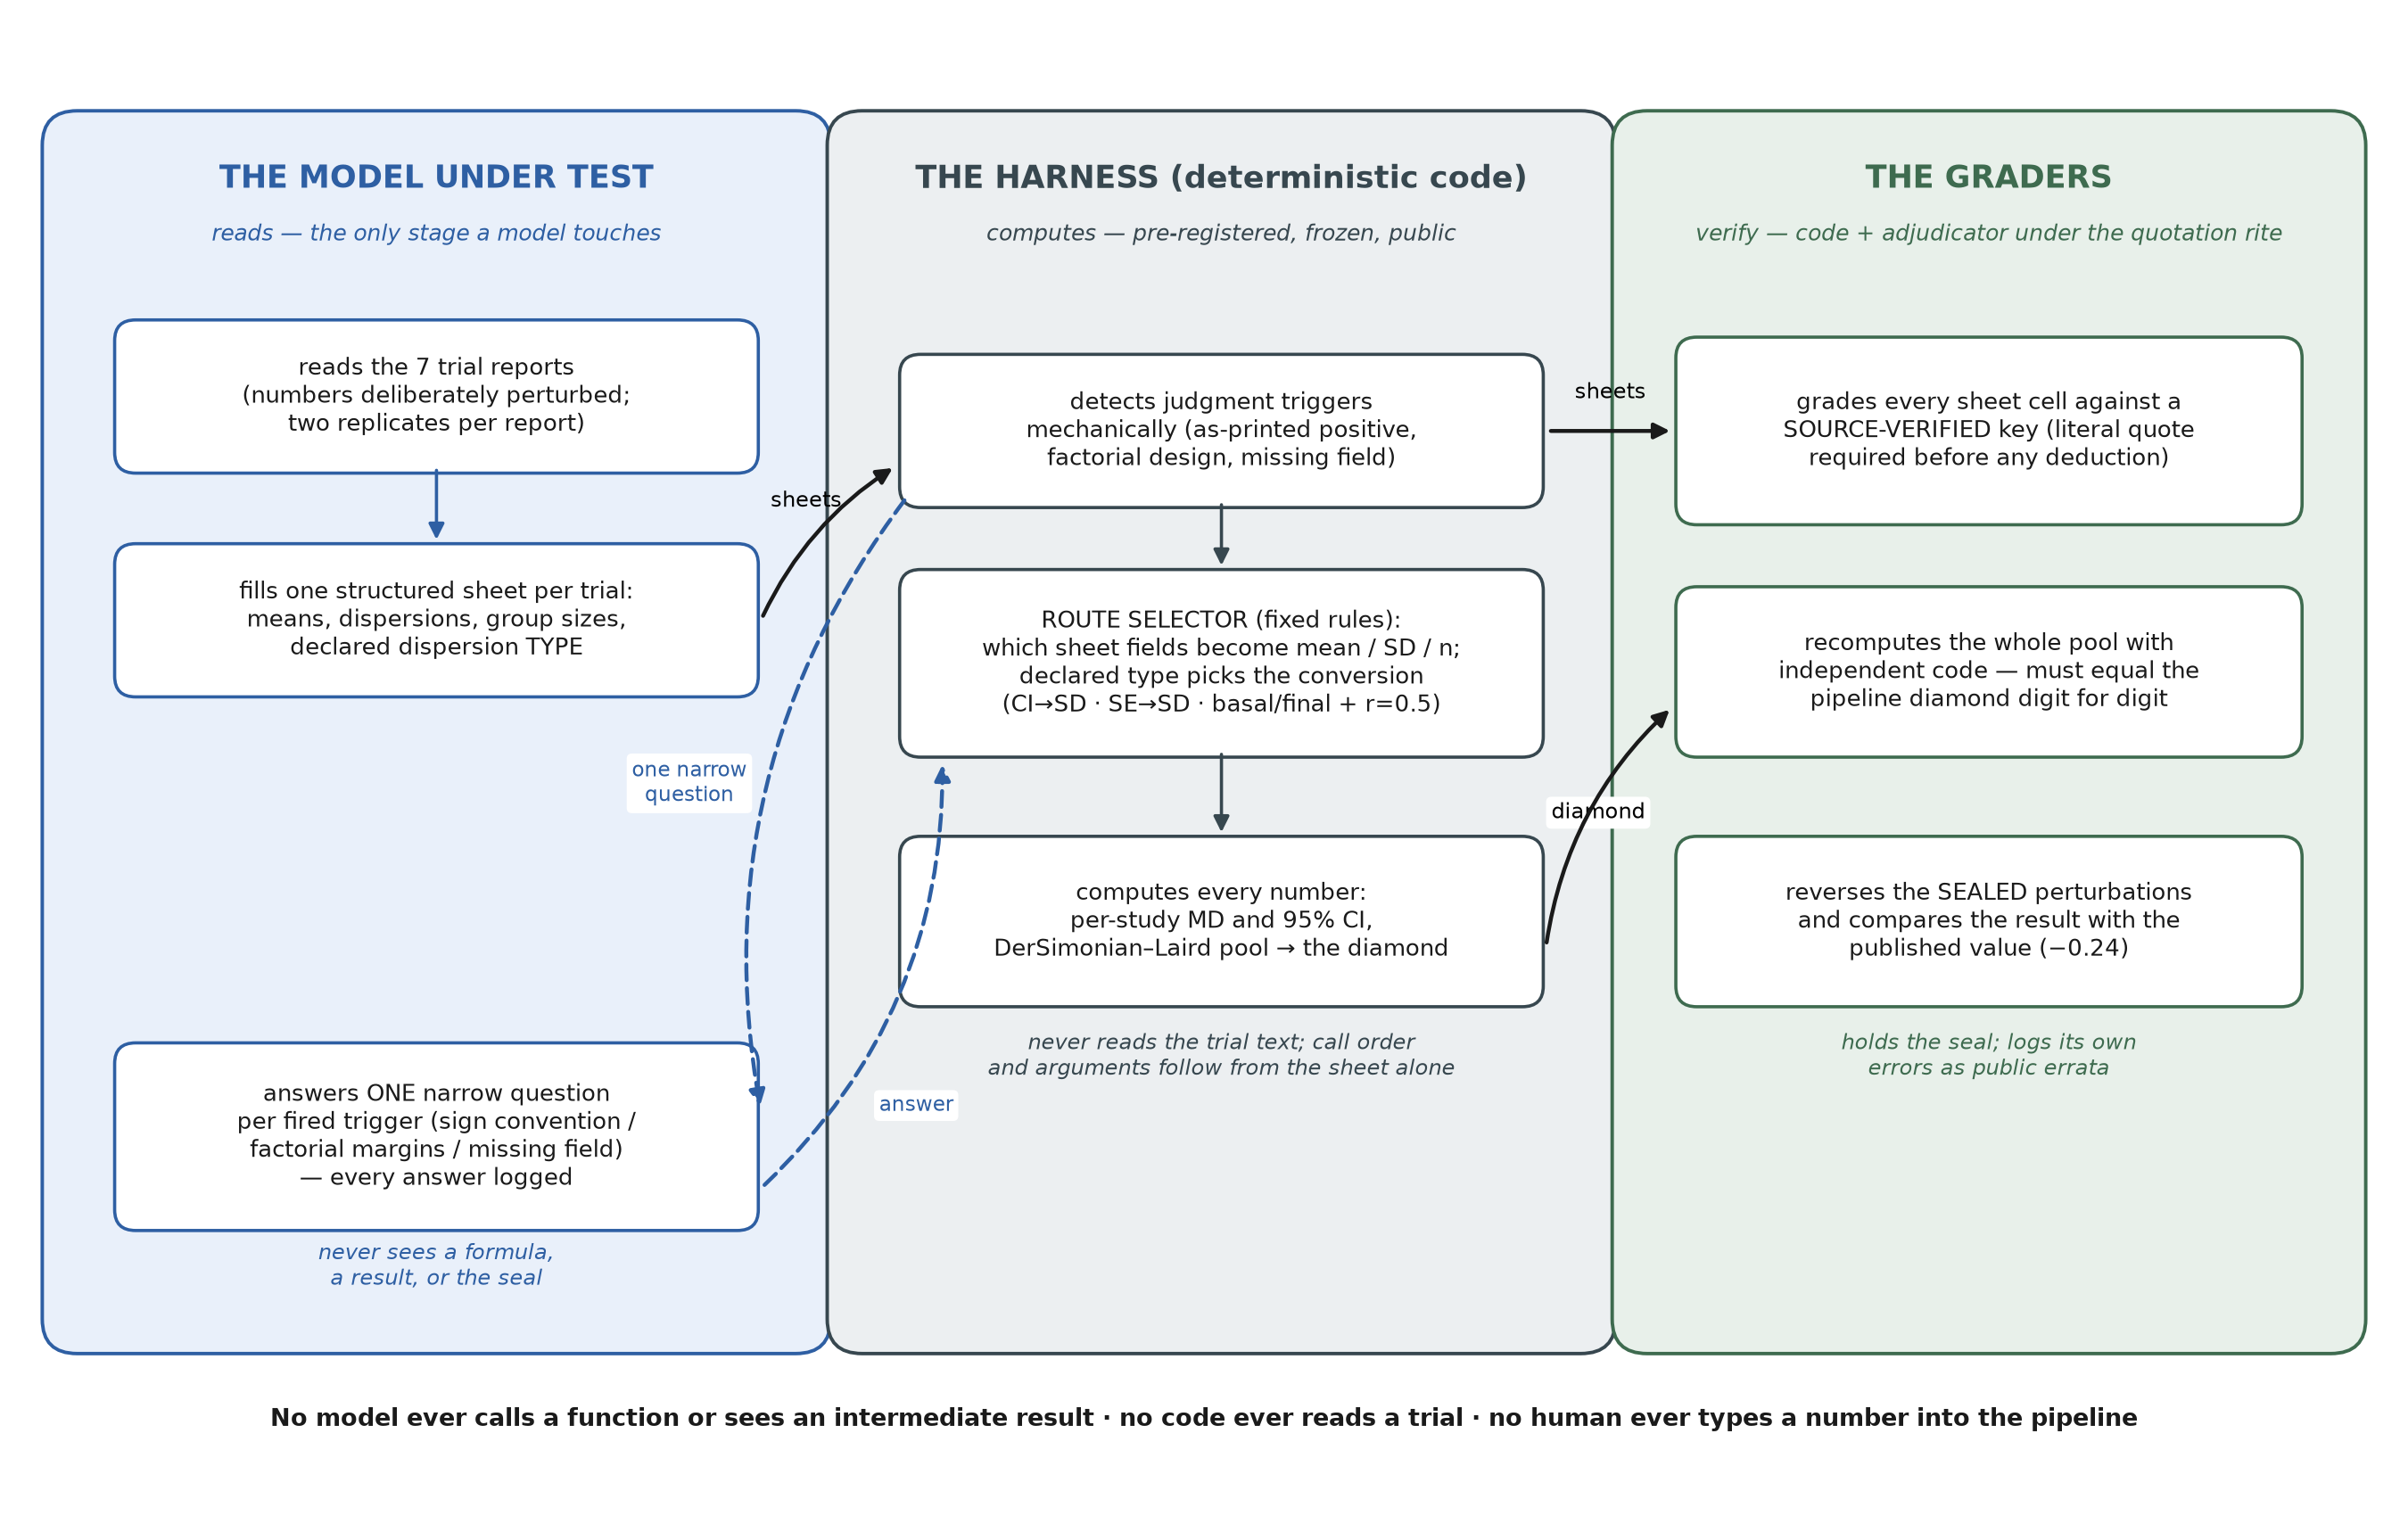
\includegraphics[width=.98\linewidth]{who-does-what.png}
\caption{Who does what. The model under test only reads: it fills one structured sheet per perturbed trial (two replicates; first parseable proceeds) and answers one narrow, logged question per fired judgment trigger. The harness --- pre-registered, frozen, public code --- detects triggers mechanically, selects field routes by the sheet's own declarations, and computes every number through validated functions (CI$\to$SD, SE$\to$SD, the Cochrane $r{=}0.5$ change-SD rule \citep{higgins2023handbook}, per-study mean differences, and the DerSimonian--Laird pool \citep{dersimonian1986meta}). The graders then verify three things independently: every sheet cell against the source-verified key; the whole pool by recomputation with independent code, which must equal the pipeline digit for digit; and the final estimate against the published value after reversing the sealed perturbations. No model ever calls a function or sees an intermediate result; no code ever reads a trial; no human ever types a number into the pipeline.}
\label{fig:whodoeswhat}
\end{figure}

\paragraph{Architecture.} Figure~\ref{fig:whodoeswhat} is the study's contract. Three judgment-trigger classes are defined, all mechanically detected on the sheet: an \emph{as-printed positive change} (the analysis convention is negative-equals-improvement, so a positive value warrants one question about its sign); a \emph{declared factorial design} (the analysis must use the margins the trial compares, not the factorial's individual cells); and a \emph{required field missing} (the model may recover a value only from its own sheet --- the reading stage is over --- else the trial leaves the pool, counted). Every firing and every answer is logged verbatim.

\paragraph{Models and rounds.} Five quantized open-weight models: the companion study's iGPU pair (\texttt{gemma4:12b}, \texttt{qwen3:14b}) and three models set aside at the original screening (\texttt{llama3.1:8b}, \texttt{qwen3.5:9b}, \texttt{deepseek-r1:14b} --- the last a reasoning distill, run like all others with the reasoning channel off). A first round ran the iGPU pair and was punctuated by environment failures on the benchmark machine (recorded in the protocol); a dated amendment then ordered a clean replication: \textbf{round 2, one uninterrupted 146-minute queue, all five models re-extracting from zero under uniform instruments}, with one model resident in memory at a time. Round 1 stands as published; round 2 is this paper's record, and round-1-versus-round-2 agreement for the iGPU pair is reported as run-to-run stability. Between the rounds, two instrument errata found in round 1's grading were fixed forward by the amendment: the sign-trigger question was rewritten neutrally (it had asserted what the printed positive meant --- a leading premise), and all three trigger classes were implemented (round 1 had only the first). This heterogeneity is named, and it produced the study's cleanest secondary result (Section~\ref{sec:ab}).

\paragraph{Six metrics, one guard each.} \emph{Cells}: every sheet field graded against the source-verified key (103 cells per replicate; flagged cells adjudicated against the sources with quotes) --- guards reading. \emph{Coverage}: how many of the seven trials yield a complete pair of arms --- guards silent waste; insufficiency is counted, never hidden. \emph{Diamond}: the pooled estimate the code computes from the model's sheets, in the perturbed world --- the product. \emph{$\Delta$ versus own-sheet truth}: the same sheets re-pooled by the graders' independent code; any gap must be named --- guards the plumbing, and proves no difference between models is arithmetic. \emph{Unperturbation lens}: the graders reverse the sealed perturbations on the sheets and re-pool; comparison with the published $-0.24$ answers the study's question --- reading errors survive this reversal, planted displacements do not. \emph{Replicate agreement}: the fraction of graded cells identical between the two independent reads --- guards luck.

\section{Results}

\begin{table}[t]
\centering\footnotesize
\setlength{\tabcolsep}{3.6pt}
\caption{Round 2 (the primary record): five extractors under the identical deterministic downstream. Cells are final, after adjudication of all 181 mechanically flagged cells against the sources (4 flips to correct, all formatting; 177 confirmed wrong). The anchor as published: $-0.24$ $[-0.32, -0.16]$, $I^2$ 6\%.}
\label{tab:round2}
\begin{tabular}{lcccccc}
\toprule
Model & Cells & Coverage & Diamond (perturbed) & $\Delta$ vs.\ truth & Lens vs.\ $-0.24$ & Replicates \\
\midrule
\texttt{gemma4:12b}     & \textbf{92.2\%} & 7/7 & $-0.52$ $[-0.82,-0.22]$ & \textbf{0.00} & $\mathbf{-0.27}$ $[-0.38,-0.17]$ & 96.1\% \\
\texttt{qwen3:14b}      & 73.3\% & 7/7 & $-0.62$ $[-0.99,-0.25]$ & 0.15$^{a}$ & $-0.51$ $[-0.74,-0.28]$ & 82.5\% \\
\texttt{qwen3.5:9b}     & 76.2\% & 6/7 & $-0.57$ $[-0.84,-0.30]$ & 0.01 & $-0.44$ $[-0.62,-0.25]$ & 63.1\% \\
\texttt{llama3.1:8b}    & 70.9\% & 5/7 & $-0.30$ $[-0.49,-0.10]$ & 0.16$^{b}$ & $-0.52$ $[-0.78,-0.25]$ & 81.6\% \\
\texttt{deepseek-r1:14b}& 67.5\% & 4/7 & $-0.43$ $[-0.64,-0.22]$ & \textbf{0.00} & $-0.54$ $[-0.75,-0.33]$ & 58.3\% \\
\bottomrule
\end{tabular}

\smallskip
\raggedright\footnotesize $^{a}$Dominated by a documented sign-doctrine overreach in the \emph{graders'} own reference code (the pipeline's judgment was correct; Section~\ref{sec:ab}). $^{b}$The values its missing-field trigger recovered from its own sheet versus the graders' routes --- instrument layer, named.
\end{table}

\begin{figure}[t]
\centering
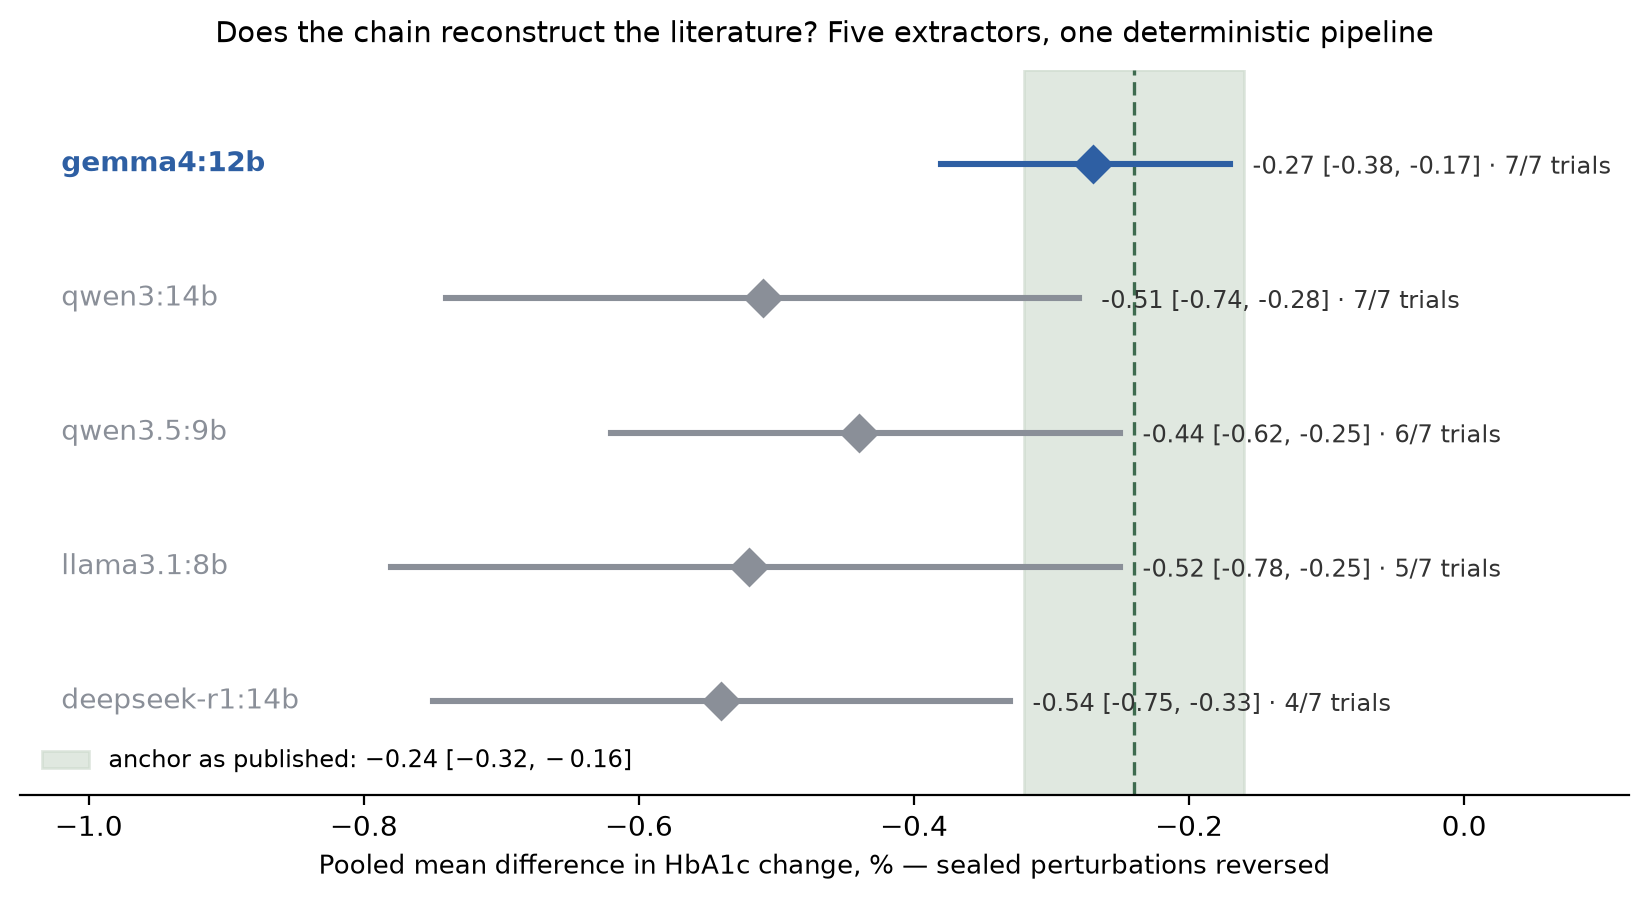
\includegraphics[width=.9\linewidth]{lens-vs-anchor.png}
\caption{The answer. For each extractor, the pooled estimate after the graders reverse the sealed perturbations on its own sheets (diamond and 95\% CI; the fraction shows how many of the seven trials its sheets supported), against the anchor's published estimate (shaded band). One extractor reconstructs the literature; four do not --- and the reversal is exactly why: it undoes what the benchmark displaced, not what a model misread.}
\label{fig:lens}
\end{figure}

\paragraph{The answer.} \textbf{Yes --- for exactly one of five} (Table~\ref{tab:round2}, Figure~\ref{fig:lens}). \texttt{gemma4:12b}, reading from zero, feeds the deterministic engine sheets whose unperturbed pool lands beside the published diamond ($-0.27$ $[-0.38, -0.17]$ vs.\ $-0.24$ $[-0.32, -0.16]$; in round 1 the same chain landed on $-0.24$ $[-0.33, -0.16]$, the published point to the hundredth). The other four extractors land between $-0.44$ and $-0.54$ --- outside or barely touching the published interval, with less of the evidence base surviving (6/7, 5/7, 4/7 trials).

\paragraph{Zero arithmetic anywhere --- and still no shared answer.} Every model's pipeline pool equals the graders' independent recomputation over the same sheets to within rounding; for \texttt{gemma4:12b} and \texttt{deepseek-r1:14b} the match is digit for digit. The two residual gaps are named and neither is arithmetic: \texttt{qwen3:14b}'s traces to the reference code itself (whose sign convention, written for one trial's printed-drop notation, over-applies to a genuinely worsened arm --- a grader-side erratum, quantified under both doctrines in the record), and \texttt{llama3.1:8b}'s to the values its missing-field trigger legitimately recovered from its own sheet by a route the reference code does not take. This is the study's structural finding: \textbf{in-world exactness and fidelity to the literature are independent axes.} \texttt{deepseek-r1:14b} is the didactic case --- perfectly exact inside its own world, and its world is wrong and half-covered. A deterministic harness does not repair bad reading; it propagates it reproducibly. Determinism, moreover, is only fully defined over well-formed sheets: on malformed cells (a CI pasted as a dispersion, a value in the wrong unit), two independently written deterministic parsers resolved the garbage differently --- parsing itself becomes a route choice, which is an argument for one shared parser, not for a model in the loop.

\paragraph{Why the four fail: a taxonomy with quotes.} Every deduction below is anchored to a source quote in the public adjudication record. \texttt{qwen3:14b} \emph{computes where the instrument says read}: it wrote CI half-widths as ``dispersions'' (values printed nowhere) and, on a trial whose table prints only baseline and final levels, wrote the changes it had itself derived. \texttt{qwen3:14b} and \texttt{qwen3.5:9b} both assembled a \emph{unit-and-level chimera} on the one trial that reports its endpoint in two units: baselines in mmol/mol, the \emph{between-group} difference placed as one arm's change, the difference's confidence interval pasted as both arms' dispersion --- every value printed somewhere, the assembly belonging to no world. \texttt{deepseek-r1:14b} extracted a \emph{printed value from the wrong timepoint} (a 3-month secondary row where the 6-month primary is required) and put total-sample baselines in per-arm fields. \texttt{llama3.1:8b} produced the benchmark's \emph{first outright inventions} --- final values and changes printed nowhere in any form (the companion study's four veterans: zero inventions in 624 cells). \texttt{qwen3.5:9b} contributed two new behavior classes: it \emph{averaged two group sizes} into ``n = 41.5'', and on one field it wrote its entire chain of reasoning \emph{into the sheet cell}. Replicate agreement adds the reliability axis: \texttt{gemma4:12b} gives the same cell 96\% of the time; \texttt{deepseek-r1:14b}, 58\% --- and notably, models can be \emph{stable in their errors}: \texttt{qwen3:14b} reproduced its chimera identically in both replicates.

\paragraph{The triggers, measured.}\label{sec:ab} The factorial-margin trigger fired for four of five models on the one factorial trial (the fifth had declared the design ``parallel'' on its sheet and escaped --- a logged escape the amendment predicted, since the trigger reads the sheet, not the source). All four models answered ``SIM'', confirming their own per-cell grouping --- which the key scores as the wrong grouping: \textbf{the trigger detects, but extractor self-verification does not correct.} The missing-field trigger fired twelve times and genuinely recovered sheet-derivable dispersions three times for \texttt{llama3.1:8b}. And the sign trigger produced the study's cleanest secondary result, an accidental A/B with one variable: in round 1, under a question that asserted ``the text prints the DROP as a positive number'' (a premise true of a different trial), \texttt{qwen3:14b} flipped a genuinely worsened control arm's $+0.3$ to $-0.3$; in round 2, under the neutral question (which states only the analysis convention), the same model, same sheet, same value, \emph{kept} $+0.3$ --- correctly. The round-1 flip was manufactured by the instrument, not by the model: \textbf{leading questions create phantom failure modes}, a caution that applies to any evaluation in which a model is asked to judge under a framing \citep{zheng2023judging}.

\paragraph{Stability.} Across two fully independent rounds, \texttt{gemma4:12b}'s diamond is identical ($-0.52$), its cells rose from 89.3\% to 92.2\%, and its replicate agreement from 89.3\% to 96.1\% --- the champion extractor is also the most stable. Its residual cell losses are route drifts, not value errors: the factorial's per-cell counts where margins are required, and an analysis-table $n$ in a randomization field on a trial whose own counts do not reconcile (92 randomized, table $n$s summing 83, 85 completing --- the primary is internally inconsistent, a finding of the companion study's kind).

\section{Discussion}

\paragraph{Division of labor as a design principle.} The measured arc across the two papers is simple: models failed at orchestration in every form offered --- spontaneous, netted, even merely arithmetical --- and succeeded at reading in exactly one case. The response that worked was not a better model but a shorter job description: \emph{everything deterministic in code; the model only where reading is irreducible; every model judgment logged as data}. Under that division, the entire between-model variance of a meta-analysis pipeline collapsed into one stage, extraction --- which is precisely the stage that can be graded cell by cell against sources. For builders of automated evidence synthesis \citep{bakker2026minutes,mclaughlin2026fully}, the practical implication is directly transferable: the fewer decisions a model makes, the fewer places an evaluation has to look, and agreement-based validation of whole chains \citep{lee2026noninferiority} cannot see the one axis that separated our five extractors --- fidelity to a source-verified, contamination-resistant reference.

\paragraph{Necessary is not sufficient.} In-world exactness --- pipeline equals recomputation --- is the correctness claim automation reports naturally make, and two of our five models achieve it perfectly while failing the question that matters. Any evaluation of a ``deterministic'' or ``tool-grounded'' pipeline should therefore report both axes separately: does the machine compute what its inputs say (plumbing), and do its inputs say something true (reading)? The unperturbation lens operationalizes the second axis at zero marginal cost once a perturbation seal exists.

\paragraph{Instruments are part of the system under test.} Round 1's leading question manufactured a sign flip; the graders' own reference code over-applied a sign convention; two deterministic parsers disagreed on malformed cells; and a trigger that reads the sheet can be escaped by a sheet that misdeclares the design. All four are instrument findings, all four are published as errata with fixes forward, and one of them was demonstrated experimentally by the A/B. Benchmarks that do not audit their own instruments will attribute instrument behavior to models --- in either direction. The perturbation seal, meanwhile, doubles as an \emph{anti-plausibility} instrument: by construction it makes the clinically expected answer the wrong one (a control arm that worsens; displaced effect sizes), so plausibility-seeking behavior --- by a model, or encoded in a grader's convention --- scores as a visible error instead of passing silently, as it would in any benchmark whose answer key points the same way as clinical expectation. Every plausibility flip caught across the two papers, genuine or instrument-made, was caught by exactly this opposition.

\paragraph{What an iGPU buys today.} The affirmative half of the answer is deployment-relevant under the privacy constraints that motivate local models in health settings \citep{wiest2024privacy,spaanderman2025openweight,flemyng2025position}: a 12B quantized model on an integrated GPU, reading from zero, plus frozen code, reconstructed a published meta-analysis end to end in a 146-minute five-model queue on a consumer mini-PC, with no cloud API anywhere. The negative half is equally practical: at this scale the extractor is not interchangeable --- four plausible substitutes, including a newer 9B and a reasoning distill, produced worlds the literature does not contain.

\section{Limitations}

One anchor, one clinical domain, one language pair, one quantization per model; the affirmative answer is one model on one corpus, and every superlative is scoped to it. The trigger set covers three declared classes and is sheet-scoped by design --- a model that misdeclares its sheet escapes detection, as one did. The graders' reference code carries two quantified errata (a sign-doctrine overreach and parser divergence on malformed cells), both reported under both readings rather than hidden; fixes apply forward, never retroactively. The two rounds differ by the amendment-registered instrument fixes, which is named heterogeneity, not silent drift; round-round stability is reported for the pair that ran twice. No formal between-model inference is attempted with $n{=}7$ trials per pool. Generalization of the frozen engine to a new anchor in a different domain is the designed next step, not a demonstrated property.

\section{Conclusion}

When a meta-analysis pipeline keeps models only where reading is irreducible, the pipeline stops failing in interesting ways and starts failing in exactly one: what the model read. That concentration is the result. It makes small local models auditable at the only stage they still own --- cell by cell, against sources, with contamination made observable --- and it makes the affirmative case concrete: one 12-billion-parameter model on an integrated GPU, given nothing but frozen code and seven perturbed trial reports, rebuilt a published meta-analysis to the hundredth. The other four rebuilt worlds that do not exist --- flawlessly.

\section*{Data and code availability}

All protocols (pre-registered, with dated amendments), frozen prompts, perturbation seals, the deterministic engine, graders, per-cell adjudications with source quotes, raw model sheets, the side-by-side reading-sheet and full-arithmetic documents, both rounds' complete records, and the exact quantized builds (pinned by Ollama digest) are public at \url{https://github.com/gbbarra/llm-evidence-extraction-benchmark-ptbr} and archived at Zenodo \citep{barra2026extrai}. Closed-stratum primary articles are not redistributed; scripts rebuild the corpus from legally obtained copies.

\section*{Declarations}

\paragraph{Funding.} This work received no external funding. All computation ran on the author's own consumer hardware; neither the author nor any institution received payments or services from a third party, in the past 36 months or otherwise, that could be perceived to influence this work.

\paragraph{Competing interests.} The author declares no competing interests. For transparency: the AI assistant acknowledged below (Claude, Anthropic) was used under an ordinary consumer subscription paid by the author, and the author has no financial or professional relationship with Anthropic or with the organizations whose open-weight models are evaluated here.

\paragraph{Ethics approval and consent.} Not applicable. This study involved no human participants and no new data collection from humans: it analyzes only published, aggregate-level reports of randomized controlled trials and a published meta-analysis. No institutional review board approval or participant consent was required.

\paragraph{Clinical trial registration.} Not applicable: no clinical trial was conducted. The randomized trials analyzed are published reports registered by their original investigators.

\section*{Acknowledgments}

This study was designed and conducted by the author with the assistance of Claude (Anthropic), which co-designed the instruments, implemented the deterministic engine, graders and queue scripts (all pre-registered and public), served as accountable adjudicator under the quotation rite --- logging four instrument errata of its own in this study --- and drafted this manuscript under the author's direction and review. The evaluated local models (\texttt{gemma4:12b}, \texttt{qwen3:14b}, \texttt{llama3.1:8b}, \texttt{qwen3.5:9b}, \texttt{deepseek-r1:14b}) produced only the extraction sheets and the logged trigger answers graded here; every downstream number was produced by the frozen code and verified mechanically. Per the RAISE-aligned position of the evidence-synthesis organizations \citep{flemyng2025position}, every AI contribution is reported and the author retains responsibility for the work.

\bibliography{references}

\end{document}
